% === PVLDB Volume 20 (VLDB 2027) -- Experiment, Analysis & Benchmark ==========
% Rules (vldb.org/2027/submission-guidelines.html, checked 2026-10-20):
%   * <= 12 pages excluding references; appendices and acknowledgements COUNT
%   * official PVLDB template (github.com/vldbproceedings/VLDB-Template, 39c95f5);
%     mandatory blocks rendered by \vldbtopmatter -- do not remove
%   * single-blind: names and affiliations on page 1
%   * title suffix "[Experiment, Analysis & Benchmark]" (removed on acceptance)
%   * EA&B: link to the full reproducibility package in the initial submission
%   * monthly deadline 1st 5pm PT, abstract by the 25th before; target 2026-12-01
% Generated from docs/icde_2027/paper.tex by experiments/scripts/port_to_pvldb.py;
% edit this file from now on.
% ================================================================================
\documentclass[sigconf, nonacm]{acmart}

%%% do not modify the following VLDB block %%
%%% VLDB block start %%%
\usepackage{pvldb}% VLDB/PVLDB formatting overrides, see pvldb.sty for details.
                      % Do not remove -- required for consistent proceedings
                      % formatting across all VLDB submissions.
%%% VLDB block end %%%

\renewcommand\vldbdoi{XX.XX/XXX.XX}
\renewcommand\vldbpages{XXX-XXX}
\renewcommand\vldbavailabilityurl{https://github.com/suanlab/sound-bounds-in-practice/tree/pvldb2027-submission-r6}

\usepackage{booktabs}
\setlength{\emergencystretch}{2em}

\begin{document}

\title{Sound Cardinality Bounds in Practice: Guards, Estimates, and Plan
Certificates [Experiment, Analysis \& Benchmark]}

\author{Suan Lee}
\orcid{0000-0002-3047-1167}
\affiliation{%
  \institution{Semyung University}
  \city{Jecheon}
  \country{Republic of Korea}
}
\email{suanlee@semyung.ac.kr}

\begin{abstract}
Sound join-size bounds are proposed as guards against bad cardinality
estimates. We measure what LpBound, SafeBound and a sampled lower bound buy
for estimates, plan certificates and execution, on STATS-CEB and JOB-light,
and find that the answer depends more on the estimator and consumer a bound
meets than on the bound. First, a guard repairs only the direction it sees:
underestimated queries range from 5\%
to 97\%, an upper bound helps only those that overestimate, and tightness
decides which it reaches; the sample behind the lower bound is worth more as an estimate than as a guard
(95th-percentile $q$-error 1.72 against 288). Second, treating plans as independent,
our pre-registered certificate certified nothing; a joint certificate
defined afterwards, accounting for shared sub-plans, certifies a plan within $2\times$ of optimal
$C_{\mathrm{out}}$ on 41\% of STATS-CEB and 52\% of JOB-light queries where
plan choice matters (25\% and 10\% samples), none without a lower bound; on
STATS-CEB, plans certified with the 10\% sample beat PostgreSQL's own where the
choice matters ($1.32\times$) until the sample is paid for. Third,
in execution the upper guard speeds up plans on the PostgreSQL estimates
published with LpBound $3.08\times$ on STATS-CEB, and the floor on JOB-light
($1.38\times$), yet guarded plans do not beat PostgreSQL's own
($0.95$--$1.06\times$ and $0.79$--$0.83\times$). For our PostgreSQL 13.1
instance's estimates guards change little ($1.01$--$1.09\times$): the bracket
sees their errors but is too wide; in a synthetic experiment, one within
$2\times$ of the truth recovers 71\% of the headroom. These small effects held
in six registered blocks on STATS-CEB. On PostgreSQL 16, guards on its own estimates
gained $1.14\times$ of a $1.40\times$ headroom, above our prediction, in one
run per version. On held-out JOB-range queries, a pre-registered test confirms four of five testable predictions, on
after-execution certificates and plan changes. We release the harness and
measurements and report our pipeline's defects.
\end{abstract}

\maketitle

%%% do not modify the following VLDB block %%
%%% VLDB block start %%%
\vldbtopmatter
%%% VLDB block end %%%


\section{Introduction}
\label{sec:intro}
Cardinality estimation errors are the main source of bad query
plans~\cite{leis2015good}, and every estimator, learned or
not~\cite{han2021cardest}, makes some. A \emph{sound} bound cannot be wrong on
its side: the true size of a join never exceeds an upper bound such as
LpBound~\cite{zhang2025lpbound} or SafeBound~\cite{deeds2023safebound}, and
never falls below the size of the same join over a sample. Such bounds have
become tight enough that one can use them, in three ways:
clamp an estimate that falls outside them (a \emph{guard}), plan on the bound
itself, or hand the interval between the bounds to a robust optimizer that
picks a plan it can certify. This paper measures what each use buys, where,
and at what cost.

We find that the answer depends more on the estimator a bound meets than on the bound.
\begin{itemize}
\item \emph{Estimates.} A guard repairs only the direction it sees, and
estimators differ: on STATS-CEB, NeuroCard underestimates 5\% of queries and
DuckDB 97\%. Tightening a sound bound decides which estimators it can reach; the sampled lower bound
is far more useful as an estimate than as a guard, and inside PostgreSQL it
costs a third of an executed exact count, a tenth on expensive sub-plans
(Section~\ref{sec:cardinality}).
\item \emph{Plan certificates.} Interval reasoning that treats plans as
independent certifies nothing, as our pre-registered study found; a joint
certificate, defined post hoc, that accounts for shared sub-plans certifies a
plan within $2\times$ of optimal $C_{\mathrm{out}}$ for 41--52\% of the
queries where the choice matters (25\% and 10\% samples), and only with a
lower bound; on STATS-CEB the plans certified with the 10\% sample run faster
than PostgreSQL's own where the choice matters, but with our sampler, sampling
for them costs more than it saves
(Section~\ref{sec:certificates}).
\item \emph{Execution.} Injected into PostgreSQL (13.1, and 16 for STATS-CEB),
guards recover large gains for
a strongly biased estimator and little for PostgreSQL's own estimates
($1.07\times$ on 13.1, $1.14\times$ on 16, one run each), whose
large errors the bracket sees but is too wide to correct (in a synthetic
experiment, a bracket within $2\times$ of the truth recovers 71\% of the
headroom); where the sample
finishes, planning on it recovers all of the headroom, but sampling
every sub-plan usually costs more than the query (Section~\ref{sec:execution}).
\end{itemize}
We claim no new estimator and no new bound. The contributions are the
measurements, a protocol that counts every query once and checks every ground
truth against the engine, and the analyses that tell the three uses apart. We
also report how our own earlier results failed (Section~\ref{sec:lessons}):
\textsc{null} defects in a counter and in degree statistics, two pre-registered
rules that could not be met (one by construction, one at our sample rate), a cost measured outside an engine, a join-order hint the engine did not
obey, and estimates read out of context. Most plan-level mechanisms we report
were analysed after the fact; a pre-registered test on held-out JOB-range
queries confirms four of five testable predictions about them, on certifying a
plan after execution and on plan changes (Section~\ref{sec:heldout}).
\section{Background and Related Work}
\label{sec:related}

\subsection{Producers: sound bounds and samples}
A cardinality \emph{certificate} for a (sub-)query $Q$ is a value that provably
bounds $|Q|$ from one side. On the upper side, the AGM bound~\cite{atserias2008agm}
and its degree-aware refinements~\cite{joglekar2018degree,abokhamis2017shannon}
bound a join from
relation sizes and maximum degrees; SafeBound~\cite{deeds2023safebound} makes
the degree-sequence bound~\cite{deeds2023degree} practical, and LpBound~\cite{zhang2025lpbound} uses
$\ell_p$-norms of degree sequences~\cite{abokhamis2024lpnorm} in an
information-theoretic linear program and is the tightest we know of (our
concurrent work under submission~\cite{lee2026lphceg} tightens it on cyclic
joins, outside the predicates of our workloads);
cardinality estimation graphs~\cite{chen2022ceg} place summary-based
optimistic estimators and pessimistic bounds in one framework; a recent overview surveys this
line~\cite{abokhamis2025pessimistic}. The pessimistic estimator of Cai et
al.~\cite{cai2019pessimistic} plans directly on such upper bounds. On the lower
side, xBound~\cite{stoian2026xbound} derives provable lower bounds from
base-table statistics, motivated by a systemic tendency of industrial systems
to underestimate, and a demonstration checks production estimators against
the bracket that xBound and LpBound form~\cite{stoian2026outofbounds}; we
measure what that bracket does to plans. A sample offers both kinds of value at once: the size of
the join over a sub-sampled relation is a sound lower bound, and scaled by the
inverse rate it is the unbiased point estimate of sampling-based join
estimation~\cite{li2016wanderjoin,zhao2018sampling,chen2017twolevel,leis2017sampling}, which
Leis et al.\ showed to be far more accurate than estimation from
statistics~\cite{leis2017sampling}.

\subsection{Consumers: guards, robust plans, certificates}
A certificate can be consumed in three ways. As a \emph{guard}, it clamps an
estimator's value when the estimate falls outside the certified side. As an
\emph{estimate}, it replaces the estimator: planning on upper bounds is
pessimistic optimization~\cite{cai2019pessimistic}, join ordering on simple
upper bounds can be competitive~\cite{hertzschuch2021simplicity}, and
PostBOUND~\cite{bergmann2023postbound} injects bounds into PostgreSQL for
that purpose. As an \emph{interval}, it feeds robust plan selection, an idea as old as
choosing a plan for a confidence level of the estimate~\cite{babcock2005robust}
or for a bounding box around it~\cite{babu2005proactive}: plan
bouquets~\cite{dutt2016bouquets} and SpillBound~\cite{karthik2016spillbound}
bound sub-optimality over a selectivity space, the minmax-regret
rule~\cite{alyoubi2015minmax} and optimality ranges~\cite{wolf2018optimality}
choose or validate a plan from cardinality intervals, and progressive
re-optimization~\cite{markl2004pop,perron2019reopt} corrects estimates after
part of a plan has run (on PostgreSQL its gains come from the re-ordered plans,
while the updated cardinalities add overhead~\cite{mu2025aqp}), and sampling-based
re-optimization~\cite{wu2016sampling} validates a chosen plan on samples;
learned optimizers choose among candidate plans while trying to avoid
regressions~\cite{doshi2023kepler,zhu2023lero}. These consumers assume an interval; the bound literature
produces one; we measure what the produced intervals let the consumers do.

\subsection{Evaluating cardinality estimation}
Leis et al.~\cite{leis2015good,leis2018looking} showed that estimation errors
propagate into plans, and the STATS-CEB benchmark of Han et al.~\cite{han2021cardest}
evaluates estimators end to end by injecting their sub-plan estimates into
PostgreSQL. Learned estimators~\cite{kipf2019learned,yang2021neurocard,%
hilprecht2020deepdb,hertzschuch2021flat,wu2021bayescard,wu2023factorjoin} are
usually judged by $q$-error~\cite{moerkotte2009preventing}, which Mandarapu
and Kunkunuru~\cite{mandarapu2026regimes} find to predict plan regret poorly.
Larger workloads such as CEB~\cite{negi2021flowloss} and
DSB~\cite{ding2021dsb} stress optimizers further; the LpBound artifact we
build on covers neither, so we do not use them. Lee et
al.~\cite{lee2023analyzing} inject cardinalities of controlled accuracy into SQL
Server to measure how plans respond, the protocol closest to our execution
level. Comparative studies of learned
estimators~\cite{wang2021ready,sun2021design,kim2022learned,chronis2024cardbench}
and of learned
optimizers~\cite{lehmann2024learned} evaluate the estimators themselves; we
evaluate what sound bounds do to their output. We follow the end-to-end
protocol for execution and report $q$-error only at the cardinality level.
\section{Experimental Setup}
\label{sec:setup}

\subsection{Benchmarks, sub-plans and ground truth}
Our primary benchmark is STATS-CEB~\cite{han2021cardest}: 146 queries over the
Stack Exchange dump, with 2--7 joined relations. JOB-light (70 queries over
IMDb) is the second. A \emph{sub-plan} of a query is a set of its relations that
PostgreSQL may join without a cross product, counting joins implied by key
equalities; we take the sub-plan lists, the true sub-plan cardinalities and the
per-sub-plan estimates from the reproducibility artifact of
LpBound~\cite{zhang2025lpbound}: 2{,}577 sub-plans on STATS-CEB and 696 on
JOB-light. Every exact count we execute ourselves in PostgreSQL agrees with the
artifact's truth (2{,}510 of 2{,}510 STATS-CEB sub-plans that finish within
120\,s, and 693 of 693 on JOB-light). Since sub-plans of one query share data, we
also count queries: every sub-plan was compared on 112 of 146 STATS-CEB and 68
of 70 JOB-light queries, none with a disagreement, which bounds the rate of
such defects among queries like these (fully counted, hence cheaper ones) at 2.6\% and 4.3\%
(one-sided 95\%); the timed-out sub-plans stay unchecked. An earlier, independent count in our own code had already been
reconciled with it, after it exposed two SQL-\textsc{null} defects of ours
(Section~\ref{sec:lessons}).

\subsection{Estimators and certificates}
\emph{Estimators.} At the level of whole queries the artifact provides up to
eight estimates per query: PostgreSQL, DuckDB, a commercial system (unnamed
in the artifact, whose code for it is not public),
NeuroCard~\cite{yang2021neurocard}, DeepDB~\cite{hilprecht2020deepdb},
FLAT~\cite{hertzschuch2021flat}, FactorJoin~\cite{wu2023factorjoin} and
BayesCard~\cite{wu2021bayescard} (six on STATS-CEB). For every sub-plan it
provides PostgreSQL's and DuckDB's estimates; to these we add the estimates of
\emph{our} PostgreSQL instance (``native''), read back with \texttt{EXPLAIN}.

\emph{Upper certificates.} LpBound and SafeBound as published in the artifact,
and the textbook max-degree bound computed by us from the filtered relations,
with \textsc{null} keys excluded from degree statistics. All three are checked
against the truth on every value we use.

\emph{Lower certificate.} On every sub-plan we execute, inside PostgreSQL, the
count of the join with its largest relation replaced by
\texttt{TABLESAMPLE BERNOULLI} at rate $r$ (default $0.10$, seed 0). The sampled
tuples are a subset of the relation, so this count $L$ is a lower bound with
probability one; $\hat L = L/r$ is the unbiased point estimate. The largest
relation is the one with most tuples before filters. We time the sampled count
against the exact count of the same sub-plan in the same engine: the exact
count runs first, then the sampled count, each twice with the second run timed
(once if the first exceeds 5\,s) and a 120\,s timeout. Running the exact count
first warms the cache for the sample, which favours the sample.

\subsection{Plan level}
\emph{Certificates.} For the 140 STATS-CEB queries with 3--7 relations we
enumerate all left-deep orders whose prefixes are connected by explicit join
predicates (1{,}560 sub-joins, 6{,}344 orders) and score them with $C_{out}$,
the sum of intermediate result sizes, with and without the final result, which
all orders share.

\emph{Execution.} We run PostgreSQL~13.1 built with the patch of the
STATS-CEB benchmark~\cite{han2021cardest} (\texttt{-O2}, no assertions) in a
container pinned to four logical cores of an Intel Xeon Gold 5218R (24\,GB
limit, 4\,GB shared buffers, GEQO and parallel workers off). We use the patch
only to read PostgreSQL's own estimate of every join as the planner computes it
inside the full query (Section~\ref{sec:pg16} repeats the STATS-CEB execution on
a stock PostgreSQL 16, read through a small extension instead); a policy's
values are injected, as in the LpBound
artifact, with \texttt{pg\_hint\_plan} \texttt{Rows} hints (commit pinned in
the artifact), one per join sub-plan, while base-table estimates stay
PostgreSQL's. Injecting PostgreSQL's own in-context estimates reproduces its
native plan on 143 of 146 STATS-CEB queries (the other three use joins missing
from the artifact's sub-plan list) and on all 70 JOB-light queries, and we
verify on every query that the injected truth reaches every join of the chosen
plan whose sub-plan is in the artifact's list. Each \emph{distinct} plan of a query is executed (policies that choose
the same plan share its time), three times, interleaved across plans, with a
300\,s timeout; we report medians. Plans run in the same order in every round,
PostgreSQL's own plan first, with no separate warm-up run, so the first round
also warms the cache; the artifact instead restarts PostgreSQL before each of
five runs and reports means.
The host is shared, so a query starts only when the host's one-minute load
average, over its 40 hardware threads, is below 60 (waiting up to 30 minutes,
and flagging the query otherwise), and we
report the true $C_{out}$ of each executed plan as a load-independent measure
of its work.

\begin{table}[t]
\centering
\caption{What each level measures, on which units.}
\label{tab:overview}
\footnotesize
\setlength{\tabcolsep}{3pt}
\begin{tabular}{@{}llrl@{}}
\toprule
Level & Unit & $n$ & Measure \\ \midrule
\multicolumn{4}{@{}l}{\emph{STATS-CEB}} \\
Estimate & query $\times$ estimator & 870 & $q$-error, under share \\
Tightness & query $\times$ estimator & 876 & $B/|Q|$, firing rate \\
Sample cost & sub-plan & 2{,}509 & sampled / exact time \\
Certificate & query (3--7 rel.) & 140 & share with $R\le2$ \\
After execution & query (3--7 rel.) & 137 & share certified $\le2$ \\
Execution & query & 146 & speedup, true $C_{out}$ \\
\multicolumn{4}{@{}l}{\emph{JOB-light}} \\
Estimate & query $\times$ estimator & 560 & $q$-error, under share \\
Sample cost & sub-plan & 693 & sampled / exact time \\
Certificate & query (3--5 rel.) & 67 & share with $R\le2$ \\
After execution & query (3--5 rel.) & 67 & share certified $\le2$ \\
Execution & query & 70 & speedup, true $C_{out}$ \\
\multicolumn{4}{@{}l}{\emph{JOB-range (held out, pre-registered)}} \\
After execution & query (3--5 rel.) & 179 & share certified $\le2$ \\
Tightness sweep & query & 191 & share of plans changed \\
\bottomrule
\end{tabular}
\end{table}

\emph{Headroom.} We call the speedup from planning on the true join sizes,
over planning on a source's own injected estimates, that source's
\emph{headroom}. It is a measured reference, not a bound: true join sizes
leave base-table estimates and the cost model as they are, and on single
queries a guard's plan can beat the truth's (by more than 10\% for the
two-sided guard on PostgreSQL 13.1, on 2 of 146 STATS-CEB queries for our
estimates, 4 for the published PostgreSQL estimates and 11 for DuckDB's). No
guard's geometric mean exceeded the headroom in any of our runs.

\subsection{Statistics}
Rows that share a query are not independent: a query contributes one row per
estimator, and plans of one query share data. We therefore report 95\%
percentile intervals from a \emph{query-clustered} bootstrap (10{,}000
replicates, seed 0) that resamples whole queries, and every plan-level
comparison counts a query exactly once. Zero counts are reported with exact
one-sided Clopper--Pearson bounds. Analyses differ in which queries they can
use: execution uses all 146 STATS-CEB and 70 JOB-light queries; the cardinality
level the 145 STATS-CEB queries whose whole-query sample finished; certificates
the 140 with 3--7 relations (138 for SafeBound) and 67 on JOB-light; planning on
$\hat L$ the 128 whose every sample finished; the sampling cost the 127 without
a timed-out sample or native plan; selective sampling the 136 with a timed
native plan; the oracle's sampling price the 57 queries certified at $r{=}0.10$;
certifying after execution 137 STATS-CEB and 67 JOB-light queries; and the guard
funnel all 146. Analyses added after we saw a result are
labelled \emph{post-hoc} where they appear.
\section{Cardinality Level}
\label{sec:cardinality}

We first ask what a certificate does to the estimate of a whole query. A
\emph{guard} returns the upper bound $B$ when the estimate $e$ exceeds it and the
lower bound $L$ when $e$ falls below it; for a sound bound every estimate beyond
it is certified wrong, so we gate at the bound itself ($\tau{=}1$; gating at
$2B$ and $L/2$ gives the same tails). We compare the guards with using a
certificate \emph{as} the estimate. Rows are the 870 (query, estimator) pairs of
the 145 STATS-CEB queries whose in-engine sample finished; the lower bound is
PostgreSQL's sampled count of the whole query.

\subsection{Which direction a guard can repair depends on the estimator}
An upper bound can only ever lower an estimate, so by construction it cannot
repair an underestimate, and a lower bound cannot repair an overestimate; what
is \emph{measured} is how much of each estimator's error lies on each side
(Table~\ref{tab:direction}). That share ranges from 5\% to 97\%. For NeuroCard,
which overestimates, the LpBound guard cuts the 95th-percentile $q$-error from
$2.6\times10^{8}$ to $1{,}135$ and the floor adds nothing; for DuckDB, which
underestimates on 97\% of queries, the upper guard changes nothing and the
floor cuts it from $304{,}835$ to $14.7$. Pooled statistics hide this, and so
does a single system: the observation that industrial systems tend to
underestimate~\cite{stoian2026xbound} holds here for DuckDB and the commercial
system (97\% and 83\% of queries), but NeuroCard and FactorJoin mostly
overestimate on STATS-CEB. JOB-light, with all eight estimators (560 pairs, 70 queries),
repeats the pattern: the underestimate share runs from 1\% (FactorJoin) to
97\% (PostgreSQL), the upper guard repairs FactorJoin ($13{,}128\to181$) and
the floor PostgreSQL ($815\to10.3$). The direction is not even fixed per
estimator: NeuroCard underestimates on 84\% of JOB-light queries and on 5\% of
STATS-CEB queries. And where an estimator is already accurate, neither guard
has anything to do: on JOB-light the tails of BayesCard, DeepDB and NeuroCard
stay below 7 and no guard changes them. A sound bound repairs only errors that
are both large and on its side.

\begin{table}[t]
\centering
\caption{Guards by estimator: share of underestimated queries and
95th-percentile $q$-error with no guard, the LpBound upper guard, and both
guards (lower: the in-engine sampled count, $r{=}0.10$); $\tau{=}1$. Rows are
ordered by the share of underestimates.}
\label{tab:direction}
\small
\begin{tabular}{@{}lrrrr@{}}
\toprule
Estimator & Under & None & Upper & Both \\ \midrule
\multicolumn{5}{@{}l}{\emph{STATS-CEB (145 queries per estimator)}} \\
NeuroCard & 5\% & $2.6{\times}10^{8}$ & 1{,}135 & 1{,}135 \\
FactorJoin & 17\% & 1{,}539 & 632 & 632 \\
PostgreSQL & 42\% & 861 & 329 & 150 \\
FLAT & 46\% & 204 & 94.4 & 43.0 \\
Commercial & 83\% & 2{,}683 & 2{,}683 & 13.4 \\
DuckDB & 97\% & 304{,}835 & 304{,}835 & 14.7 \\
\midrule
\multicolumn{5}{@{}l}{\emph{JOB-light (70 queries per estimator)}} \\
FactorJoin & 1\% & 13{,}128 & 181 & 181 \\
FLAT & 27\% & 5.42 & 5.42 & 4.83 \\
BayesCard & 47\% & 4.84 & 4.84 & 4.84 \\
Commercial & 54\% & 65.1 & 61.7 & 12.0 \\
DeepDB & 64\% & 3.55 & 3.55 & 3.55 \\
DuckDB & 83\% & 18{,}052 & 15{,}858 & 63.0 \\
NeuroCard & 84\% & 6.97 & 6.97 & 6.97 \\
PostgreSQL & 97\% & 815 & 815 & 10.3 \\
\bottomrule
\end{tabular}
\end{table}

\subsection{A tighter bound reaches more estimators}
On all 146 queries and the same estimators, gated at the bound itself
($\tau{=}1$), the max-degree bound is a median $1{,}423\times$ above the truth,
SafeBound and LpBound $29.9\times$ and $30.8\times$; per query, LpBound is a
median 24 times tighter than max-degree. Pooled, the tighter bound fires 2.7
times as often (22.3\% of (query, estimator) pairs against 8.2\%), always
helpfully, as a sound clamp must. Pooling hides what tightness buys
(Table~\ref{tab:tightness}): max-degree fires almost only on NeuroCard, whose
overestimates are extreme, while LpBound also reaches the moderate
overestimates of PostgreSQL, FLAT and FactorJoin, which the looser bound never
touches. The firing rate is also capped by the share of overestimates, so a
ratio of firing rates understates the difference. SafeBound and LpBound are
indistinguishable in what they change.

\begin{table}[t]
\centering
\caption{Firings of each sound upper bound per estimator (146 STATS-CEB
queries each; gate at the bound). Rows ordered as in
Table~\ref{tab:direction}.}
\label{tab:tightness}
\footnotesize
\begin{tabular}{@{}lrrr@{}}
\toprule
Estimator & max-degree & SafeBound & LpBound \\ \midrule
NeuroCard & 68 & 101 & 100 \\
FactorJoin & 3 & 31 & 34 \\
PostgreSQL & 0 & 33 & 33 \\
FLAT & 1 & 22 & 27 \\
Commercial & 0 & 1 & 1 \\
DuckDB & 0 & 0 & 0 \\
\bottomrule
\end{tabular}
\end{table}

\subsection{The sample is worth more as an estimate than as a guard}
Pairing both guards cuts the pooled tail by two orders of magnitude
(Table~\ref{tab:asestimate}), but the instrument behind the floor does far
better on its own: the scaled sample $\hat L$ has a 95th-percentile $q$-error of
$1.72$, against $288$ for the best guard, and even the sound count $L$, which
sits about $1/r$ below the truth, has a tail of $16.7$. LpBound used as the
estimate (pessimistic planning's input) has a median $q$-error of 29.1 against
9.00 for guarding with it, and a tail ten times that of both guards together
(2{,}862 against 288), though below that of the upper guard alone (4{,}733).
On JOB-light the sample does as well ($\hat L$ reaches $1.22$ [1.13, 1.60]
against $19.0$ for the best guard), but it is not infallible: on two STATS-CEB
queries the result hinges on a few tuples of the sampled relation and none is
drawn, so $L=\hat L=0$ and the $q$-error equals the true size ($5{,}091$ and
$224$). What decides the choice is whether the sample's cost can be paid.

\begin{table}[t]
\centering
\caption{Guards versus certificates used as the estimate (870 pairs, 145
queries; 95\% query-clustered intervals).}
\label{tab:asestimate}
\small
\begin{tabular}{@{}lrr@{}}
\toprule
Policy & Median & 95th percentile \\ \midrule
No guard            & 16.8 & 109{,}640 [29{,}719, 463{,}853] \\
Upper guard (LpBound) & 9.00 & 4{,}733 [2{,}795, 17{,}257] \\
Upper and lower guard & 8.83 & 288 [96, 648] \\
LpBound as estimate & 29.1 & 2{,}862 [958, 15{,}865] \\
Sound $L$ as estimate & 10.0 & 16.7 [12.6, 42.3] \\
$\hat L = L/r$ as estimate & 1.03 & 1.72 [1.37, 4.23] \\
\bottomrule
\end{tabular}
\end{table}

\subsection{In the engine, sampling is cheapest where it matters}
\begin{figure}[t]
\centering
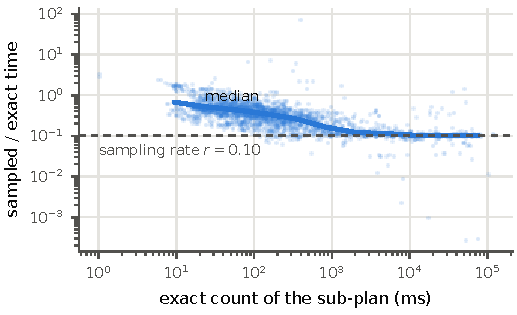
\includegraphics[width=\columnwidth]{../../figures/icde_cost.pdf}
\Description{Log-log scatter plot, one point per STATS-CEB sub-plan: the time of the sampled count divided by the time of the exact count, against the exact count's time in milliseconds, with a median line; the ratio falls from about one half on fast sub-plans to the sampling rate 0.10 on slow ones.}
\caption{Cost of the sampled count relative to the exact count of the same
sub-plan, inside PostgreSQL (2{,}509 STATS-CEB sub-plans; line: median per
logarithmic bin). On expensive sub-plans the ratio approaches the rate.}
\label{fig:cost}
\end{figure}
Measured inside PostgreSQL against the executed exact count of the same sub-plan
(Figure~\ref{fig:cost}), the sampled count costs a median $0.33\times$ [0.31, 0.36] over 2{,}509 sub-plans,
and the ratio falls as the join gets expensive: $0.48$ when the exact count
takes under 100\,ms, $0.28$ up to 1\,s, $0.12$ up to 10\,s and $0.10$ beyond,
close to the rate itself. Sampling the largest relation shrinks every
intermediate result it takes part in, which an earlier measurement of ours in a single-threaded
Python counter could not show (it reported $0.66$; Section~\ref{sec:lessons}).
\subsection{How much to sample}
Raising the rate from $0.10$ to $0.25$ raises the cost and the accuracy
together (Table~\ref{tab:rate}). On the same 548 sub-plans of 58 queries, timed while
the host was quiet, the sampled count costs a median $0.56\times$ the exact
count instead of $0.35\times$, and on sub-plans whose exact count takes over a
second $0.25\times$ instead of $0.10\times$: there the cost is the rate. The
sound count stays about $1/r$ below the truth (median $q$-error 3.98 against
10.04), $\hat L$ tightens only a little
(95th percentile 1.56 against 1.72), and the share of queries with a certified
plan rises from 40.7\% to 55.0\% (Section~\ref{sec:certificates}). The
$r{=}0.25$ run shared the host with heavy jobs for most of its duration; its
counts are valid, but we use its timings only where the load stayed below 60.
All sample-based results use one Bernoulli draw (seed 0) shared by every query,
so we repeated the $r{=}0.10$ samples with four more seeds: across the five
draws, $\hat L$'s 95th-percentile $q$-error ranges from 1.35 to 2.05, the best
guard's from 250 to 288, the sound count's median from 9.88 to 10.05, and the
share of queries with a certified plan from 40.0\% to 41.4\%. These
$r{=}0.10$ results do not rest on the draw; we did not repeat the $r{=}0.25$
samples or any execution with other draws.

\begin{table}[t]
\centering
\caption{Sampling rate on STATS-CEB: in-engine cost (median sampled / exact
time; matched quiet-host sub-plans, all and those whose exact count exceeds
1\,s), median $q$-error of the sound count $L$, 95th-percentile $q$-error of
$\hat L$ (both as the whole-query estimate), and the share of queries with a
certified plan (LpBound, joint, $\le2\times$).}
\label{tab:rate}
\footnotesize
\setlength{\tabcolsep}{3pt}
\begin{tabular}{@{}lrrrrr@{}}
\toprule
$r$ & Cost & Cost ($>$1\,s) & $L$ med. & $\hat L$ p95 & Certified \\ \midrule
$0.10$ & 0.35 & 0.10 & 10.04 & 1.72 & 40.7\% \\
$0.25$ & 0.56 & 0.25 & 3.98 & 1.56 & 55.0\% \\
\bottomrule
\end{tabular}
\end{table}

\section{Plan Level: Certificates}
\label{sec:certificates}

A sound bracket $L(S)\le|S|\le B(S)$ on every sub-plan $S$ is an interval on
every plan's cost. We ask what it can \emph{prove} about the plan a consumer
picks: a regret bound $R(p)$ with $C(p)/\min_{p'}C(p')\le R(p)$ for the true
cost $C$, from the bracket alone. Our certificates assume every sub-join is
non-empty: they floor sizes at 1, and a sample that times out contributes
$L{=}1$. That holds on every sub-join we certify (smallest true size 26 on
STATS-CEB and 2 on JOB-light, smallest exact count 1 on JOB-range); where joins can be empty, the floor
must be 0, or flooring at 1 can certify a plan of regret 3 within $2\times$ (a
test in the supplement).

\subsection{Two certificates from one bracket}
Write $C_{lo}(p)$ and $C_{hi}(p)$ for a plan's cost with every sub-plan at its
lower or upper bound. The simplest certificate is
\begin{equation}
G = \max_{p\in\mathcal{S}} C_{hi}(p) \,/\, \min_{p'} C_{lo}(p'),
\end{equation}
over the plans $\mathcal{S}$ that survive dominance pruning
($C_{lo}(p)>\min_{p'}C_{hi}(p')$ prunes $p$). It treats the two plans as if
their costs were independent, yet left-deep orders share sub-plans: under
$C_{out}$ every order shares the final result, and many share a prefix. A shared
sub-plan cannot sit at $B$ in the numerator and at $L$ in the denominator at
once. The tightest bound the same bracket supports is the joint one,
\begin{equation}
R(p) = \max_{p'}\ \max_{s\in[L,B]}\ C(p,s)/C(p',s).
\end{equation}
For a pair, write $C(p,s)=A+\mathit{Sh}$ and $C(p',s)=D+\mathit{Sh}$, with $A$
the sub-plans only $p$ uses, $D$ those only $p'$ uses and $\mathit{Sh}$ the
shared ones. The ratio is largest
with $A$ at $B$, $D$ at $L$, and the shared total at one of its two extremes,
because $(a+x)/(d+x)$ is monotone in $x$; dominance cancels shared sub-plans in
the same way ($p$ is never optimal if $A$ at $L$ exceeds $D$ at $B$ for some
$p'$). Both are exact and cost one pass over plan pairs. The joint bound is the
classical worst-case relative regret of interval-data robust
optimization~\cite{kouvelis1997robust,averbakh2005relative}; what we add is
its evaluation with intervals that are actually sound.

\subsection{What we pre-registered, and why it failed}
We pre-registered a plan-certificate study on $G$ (an internally frozen
protocol, dated before the run and included in the supplement, but not
deposited with a public registry; rule: a query is
\emph{certified} if one plan survives, \emph{useful} if $G\le2$; nine brackets,
primary LpBound $\times$ sample at $r{=}0.25$, the sample drawn by our own
Python sampler; the analyses after it use PostgreSQL's). Every verdict came
out null:
0 of 140 queries on either rule, for two different reasons we did not see when
we froze them. The first rule is unattainable by construction: under $C_{out}$
an order and the order that swaps its first two relations have equal cost under
every bracket, so at least two plans always survive (in the run, every survivor
set had even size, never below two). The second failed at our sample rate, not
by construction: with a sampled floor $L\approx r|S|$ on every sub-plan,
$G\ge C_{hi}(p^*)/C_{lo}(p^*)\gtrsim 1/r=4$ whatever the upper bound, and the
smallest $G\cdot r$ over all queries is $0.98$; $G\le2$ needs every plan's
floor cost to reach half the largest surviving upper-bound cost, which a 25\% sample
reaches only by an unlikely draw. The nulls were properties of the statistics
(the first at any rate, the second at this one), not of the brackets.

\subsection{The joint certificate (post-hoc)}
\label{sec:joint}
\begin{figure}[t]
\centering
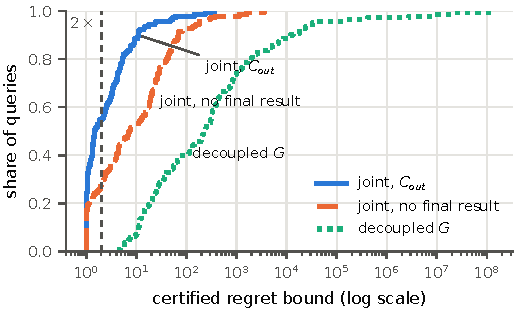
\includegraphics[width=\columnwidth]{../../figures/icde_certificates.pdf}
\Description{Cumulative distributions over 140 STATS-CEB queries of the certified regret bound on a log scale, for the joint certificate with and without the shared final result and for the decoupled G; a dashed line marks the threshold 2, which the joint certificate reaches for far more queries than G.}
\caption{Certified regret bound per query, LpBound $\times$ in-engine sample ($r{=}0.25$),
140 STATS-CEB queries: the decoupled $G$ against the joint certificate, with and
without the final result that all plans share. Post-hoc.}
\label{fig:certificates}
\end{figure}
Table~\ref{tab:certificates} and Figure~\ref{fig:certificates} report the
joint certificate on the same 140 queries, now with PostgreSQL's in-engine
sampled count as the floor (a sample that times out contributes $L{=}1$,
which can only lower the shares and is sound because these sub-joins are
non-empty). At $r{=}0.25$, LpBound certifies a
plan within $2\times$ of optimal on 55.0\% of queries (median certified bound
$1.47$) and prunes a third of all orders, against $2.7\%$ under $G$; every
plan it certifies has a true regret of at most $1.03$. At $r{=}0.10$ the share
falls to 40.7\%: the floor sits about $1/r$ below the truth, and a lower rate
loosens every certificate. These shares count every query, including the
50.7\% on which every left-deep order is already within $2\times$ of the best
in true $C_{out}$, so that any plan would do. On the 69 queries where the choice
matters (a classification that uses the true sizes and serves this analysis
only), the certificate covers 40.6\% [29.0, 52.2] at $r{=}0.25$ and 30.4\% at
$r{=}0.10$. A certificate that ignores plan structure certifies nothing:
planning on the geometric midpoint of every bracket bounds each intermediate
result's $q$-error by $q=\max_S\sqrt{B(S)/L(S)}$; Moerkotte et
al.~\cite{moerkotte2009preventing} bound the regret of such a plan by $q^4$ for
general cost functions, and for $C_{out}$ the same argument gives $q^2$, but
$q^2$ exceeds 2 on every query (median 180). Without a lower bound
($L\equiv1$) no upper bound certifies any query: the lower bound is what makes
plan certification possible, the reverse of what $G$ suggested. Two caveats
bound the claim. The shared final result, a constant every plan pays, carries
much of the effect: excluding it halves the certified share (27.9\%). And the
analysis was designed after the null and uses the plan-cost model, not
execution. SafeBound's published values fall below the truth on three
sub-joins of two queries, which we exclude from its rows (138 queries; we have
not traced the cause); on the same 138, LpBound certifies 55.1\%. Merging
each order with its first-two swap and re-applying the registered rules
certifies 5 of 140 queries, $3.6\%$ [0.7, 7.1], still below the registered bar.
Re-applying the registered paired comparison to the merged classes gives the
sampled lower bound a difference of $3.6$ points [0.7, 7.1]; it rests on 5
discordant queries (exact sign test $p=0.0625$), and we do not count this
post-hoc re-score as a registered result.

The pattern repeats on JOB-light (67 queries with 3--5 relations, in-engine
samples at $r{=}0.10$, no max-degree bound): LpBound certifies a plan within
$2\times$ of optimal for 52.2\% [40.3, 64.2] of queries and SafeBound for
37.3\% (on the 63 queries where the choice matters, LpBound certifies
52.4\% [39.7, 65.1]), every certified plan is in fact optimal, no upper bound certifies any
query without a lower bound, and without the shared final result only 10.4\%
remain. On these star-shaped joins the final result carries even more of the
effect than on STATS-CEB. The threshold 2 is a convention (post-hoc).
Certifying within $t\times$ among the queries whose true spread exceeds $t$,
LpBound covers 35.6\%, 45.5\% and 54.3\% of STATS-CEB at $r{=}0.25$ for
$t=1.5$, 3 and 4, a smooth trend, and 28.8\%, 64.2\% and 71.1\% of JOB-light
against 52.4\% at 2; on JOB-light's fixed 63 queries it certifies 19 at
$t=1.5$ against 33 at 2, so many of its certificates lie between 1.5 and 2.

\subsection{What makes a plan certifiable (post-hoc)}
The joint bound has an exact reading. With $A$, $D$ and $\mathit{Sh}$ the sets
of the pair formula for $p$ and $p'$, and $B(X)$ and $L(X)$ the sums of the
bounds over a set $X$:

\begin{proposition}
For $t\ge1$, $R(p)\le t$ if and only if, for every $p'$,
$B(A) \le t\,L(D) + (t-1)\,L(\mathit{Sh})$.
\end{proposition}

\noindent Where a pair's ratio exceeds 1 it is largest with the shared
sub-plans at $L$, which gives the condition; where it does not, the condition
holds anyway. The upper bound of what the chosen plan does alone must be paid
for by $t$ times the floor of what the competitor does alone and $t-1$ times the
floor of what the two share. Two consequences follow. First, the certificate
does not change when every floor and every upper bound are scaled by one
factor, so raising all floors $f$-fold is worth exactly cutting all upper bounds
$f$-fold. The $r{=}0.25$ sample raises the floors a median $2.51\times$ over
$r{=}0.10$ and certifies the same share of queries, 55.0\%, as dividing every
LpBound value by 2.5 at $r{=}0.10$. That cut, however, is not sound: it falls
below the truth on 658 of 1{,}560 sub-joins. Even clipped at the truth, the
tightest a bound of that form can be, it certifies only 50.7\%,
and a sound tightening that shrinks the whole-query bound $2.5\times$
geometrically certifies only 45.0\%, where our frozen prediction expected 55\%.
A sound upper bound gains only what its looseness on the deciding sub-joins
allows. Second, every plan shares the final result, whose floor therefore pays
for every pair. At $r{=}0.10$, let
\begin{equation*}
\rho = \frac{L(\text{final})}{L(\text{final}) + B(\text{non-final joins of } p_{hi})},
\end{equation*}
with $p_{hi}$ the plan with the smallest $C_{hi}$. By the
proposition, $\rho\ge1/2$ certifies $p_{hi}$ within $2\times$ (41 STATS-CEB and
17 JOB-light queries, all certified, as the proposition guarantees). As a score, $\rho$ separates certified
from uncertified queries with an AUC of 0.93 [0.88, 0.98] on STATS-CEB and 0.93
[0.87, 0.98] on JOB-light (the threshold chosen on STATS-CEB classifies 82\% of
JOB-light queries correctly), where the number of relations alone gives 0.87
and 0.64. Certification also fades with query size, on STATS-CEB from 94\% of
3-relation queries to none of the four with 7 relations. On JOB-light, where
certification also falls with size, $\rho$ stays flat across sizes, so size
matters beyond the weight of the final result.

\subsection{Does a certificate need every lower bound? (post-hoc)}
A certificate does not need a sample on every sub-join, only on those that
separate the plan it certifies from its strongest competitor. We simulated a
\emph{certify-then-stop} rule offline from the in-engine measurements at
$r{=}0.10$. Start from LpBound and $L\equiv1$; repeatedly take the plan $p^*$
with the smallest joint bound $R$ and the competitor that attains it, sample
that competitor's unsampled sub-join with the largest upper bound, charging its
measured sampling time, and stop once $R(p^*)\le2$. The rule gives up early
when even setting every unsampled $L$ to its $B$, the most any sample could
reveal, leaves $R(p^*)>2$; this test is sound, so giving up never loses a
certificate. The order of sampling depends only on $B$, the samples drawn so far
and the plans' structure, never on the truth.

It certifies exactly the queries that sampling every sub-join certifies,
40.7\% [32.9, 48.6] of 140, after sampling a median 29\% of the sub-joins, and
gives up on 55\% of queries; every plan it certifies has a true regret of at
most 1.01. Its cost, relative to the time PostgreSQL takes to execute its own
plan for the query in the execution run (136 queries), is a median
$0.44\times$ [0.36, 0.62], against $0.88\times$ [0.71, 1.32] for sampling all
1{,}560 sub-joins the left-deep orders use ($0.32\times$ on the certified
queries). Sample and execution times come from different runs, and the
execution run timed PostgreSQL's native plans $1.24\times$ and $1.33\times$
slower (geometric mean) than the two other runs that executed them; with their
times, selective sampling costs $0.53\times$ and $0.59\times$, and sampling
all sub-joins $1.24\times$ and $1.30\times$. Most of the gap comes from the 19
queries that started under high load in the execution run ($2.57\times$ and
$2.69\times$ there, $1.10\times$ and $1.18\times$ on the rest). Selective
sampling thus stays
below the query's own time under every reference; sampling every sub-join does
not. Whether the certificate is worth obtaining is the next question.

\subsection{Do certified plans run fast?}
A certificate is a statement about the cost model it is computed in, so we ran
the certified plans. We forced each certified left-deep order into PostgreSQL by
writing its joins explicitly in that order with \texttt{join\_collapse\_limit}
set to 1, which fixes the join order and leaves join methods and the inner and
outer side of each join to the optimizer, and checked every executed plan
against its order (57 certified STATS-CEB queries at $r{=}0.10$, three
interleaved runs). As controls we forced the left-deep order that is optimal in
true $C_{out}$ on all 140 queries and, on the 118 whose native plan is
left-deep, the native plan's own order. Forcing alone costs a little: the
native order, forced, runs $0.89\times$ [0.81, 0.97] as fast as the native
plan, because on 50 of the 118 queries PostgreSQL then chooses other join
methods or sides ($0.76\times$ there, $1.01\times$ on the rest). Yet the
$C_{out}$-optimal order runs $1.15\times$ [1.02, 1.31] as fast as the native
plan ($1.20\times$ [1.08, 1.38] against the forced native order), and the
certified orders $1.07\times$ [0.94, 1.23] (faster on 35\% of queries, slower
on 11\%). On 52 of the 57 certified queries the certified order is the
$C_{out}$-optimal order itself, so the certificate finds the order that is
best in $C_{out}$, and that order is a good one for PostgreSQL. The average
mixes two kinds of query. Where the choice matters (21 queries; a post-hoc
split), the certified plans run
$1.32\times$ [1.10, 1.63] as fast as the native plan; where every order is
within $2\times$ of the best (36), $0.95\times$ [0.80, 1.11]. What
certification costs is the sample: charging the time of the selective sampling above, the certified
plans run $0.56\times$ [0.42, 0.72] as fast as the native plan, and
$0.34\times$ [0.17, 0.57] where the choice matters (sample times from the
sampling run). Among the samples we measured, no choice of which to take would
make the certified plans, sampling included, faster than the native plan on
average (post-hoc). We computed exactly, by branch and bound, the least sampling time
with which any subset of the measured samples would have certified each query
(feasibility is monotone in the set sampled, since the joint bound can only fall
as floors rise): selective sampling already pays this price on 77\% of the 57
certified queries (62\% of the 21 where the choice matters). Charged the
oracle's price instead of the online rule's, the same executed plans still run
$0.67\times$ [0.52, 0.81] as fast as the native plan over the 57 queries and
$0.51\times$ [0.28, 0.78] where the choice matters, faster on 14\% of those.
Our frozen prediction that even this price would exceed the query's execution
time on half of those queries failed (19--33\%): the oracle's sampling alone is
cheaper than the query on most of them, but not cheap enough to pay for
itself. Nor is a floor of another kind cheaper here: witnessing the same floors
with $k$ result tuples of the exact join (\texttt{LIMIT} $k$, so $k$ is the
sampled count, about a tenth of the join, not the smallest floor the
certificate needs, which our frozen prediction named), which stops as soon as it
has them, costs a median $0.96\times$ [0.80, 1.04] of the sampled count of the
same sub-join (70 sub-joins, timed back to back), against our frozen prediction
of at most $0.2\times$. The certificate is cheap in plan quality and expensive in
sampling, at least with our sampler (largest relation, fixed rate, charged per
sub-plan) and the plans we executed; choosing samples and plans jointly, or a
statistics-based floor, we did not evaluate.

\subsection{Certifying after execution (post-hoc)}
A consumer need not certify before it runs a plan. Once PostgreSQL has executed
its own plan, every intermediate size of that plan is known exactly; with those
sizes (here the exact sizes of our ground truth, standing in for what an
instrumented execution would report; we did not instrument one) and a floor on every other sub-join, the executed plan's regret over
the left-deep orders is soundly at most $C(p)/\min_{p'}C^{p}_{lo}(p')$, where
$C^{p}_{lo}$ takes each sub-join at its exact size if $p$ computed it and at its
floor otherwise. No upper bound enters: the plan's own exact sizes are the
tightest possible lower bounds, the final result among them. The competitors
remain the left-deep orders over explicit join predicates, also where
PostgreSQL's plan joins through an implied equality (31 queries). At $r{=}0.10$ this
certifies PostgreSQL's plan within $2\times$ on 86.1\% [80.3, 91.2] of 137
STATS-CEB queries (three lack sub-plan truth; 89.1\% are in fact within
$2\times$), but that needs a sample of every sub-join the plan did not compute;
with no sample at all, the exact sizes alone certify 83.9\% [77.4, 89.8]. On
JOB-light the shares are 100\% and 97.0\% of 67. These certificates rest on the
final result, as before execution (Section~\ref{sec:joint}): without it, the
certificate covers 21.2\% of STATS-CEB and 41.8\% of JOB-light plans with the
sample and almost none without it (0\% and 1.5\%), although 67.9\% and 86.6\%
are in fact within $2\times$ in that cost. A certificate after the fact can tell
a learned optimizer to stop exploring a query or vouch for a cached plan; under
$C_{out}$ with the final result it says only that the work before the output is
small.

\begin{table}[t]
\centering
\caption{Share of 140 STATS-CEB queries whose bracket certifies a plan within
$2\times$ of optimal (joint certificate, left-deep orders; floor: PostgreSQL's
in-engine sampled count at $r{=}0.25$, last column $r{=}0.10$; 95\% intervals
over queries; SafeBound rows over 138 queries). Post-hoc.}
\label{tab:certificates}
\footnotesize
\setlength{\tabcolsep}{3pt}
\begin{tabular}{@{}llrrrr@{}}
\toprule
Upper & Lower & $\le2\times$, $C_{out}$ & med.\ $R$ & no final & $r{=}0.10$ \\ \midrule
LpBound & sample & 55.0\% [46.4, 62.9] & 1.47 & 27.9\% & 40.7\% \\
SafeBound & sample & 56.5\% [47.8, 64.5] & 1.45 & 28.3\% & 42.8\% \\
max-deg. & sample & 35.7\% [27.9, 43.6] & 8.59 & 17.1\% & 29.3\% \\
any & $L\equiv1$ & 0\% & ${\ge}1.4{\times}10^{5}$ & 0\% & 0\% \\
\bottomrule
\end{tabular}
\end{table}
\section{Plan Level: Execution in PostgreSQL}
\label{sec:execution}

Certificates and $q$-errors are proxies; we now execute. For each query and
each policy we inject the policy's value for every join sub-plan into
PostgreSQL, let it plan, and run the plan (Section~\ref{sec:setup}). Each
benchmark is measured in a single run that covers every estimate source and
policy, so all numbers in a table share one host state (median one-minute load
at query start 4.9 on STATS-CEB and 2.9 on JOB-light; the load gate flagged no
query, though 19 STATS-CEB queries, in one stretch of 22, started at a load
above 30). Speedups are geometric means over queries, one row per query, with
query-clustered intervals; a query counts as faster or slower only when the
ratio leaves a $\pm10\%$ band. Every plan is timed three times except those that
hit the 300\,s timeout (25 plans on STATS-CEB and 11 on JOB-light), which are
kept at 300\,s, so every speedup is one of capped runtimes. Where only the
baseline's plan times out, a query's capped ratio is a lower bound on its
speedup; where only the policy's does, an upper bound. The latter happens
mostly when a biased source's plan, guarded or not, is set against the native plan, where it
understates a slowdown; for a policy over its own source's estimates it happens
on one DuckDB query on 13.1, one synthetic-bracket query on PostgreSQL 16 and
one query of the forced native order (Section~\ref{sec:certificates}).
Where two different plans both time out (at most five queries in any
comparison) the ratio enters as 1 with unknown direction. Leaving those
queries out moves no geometric mean of any executed run by more than 5\%
(post-hoc; every comparison's cases are in the supplement). Neither the cap nor the load
drives the results: with every time re-capped at 120\,s or 60\,s, or without
those 19 queries (the upper guard's $3.08\times$ then becomes $2.76\times$),
every geometric mean below that lies more than 2\% from parity keeps its
direction; a 5\% or 20\% band changes the sign of the balance of faster and
slower queries only on three comparisons within $1.10\times$ of parity.
Intervals are over queries within one run; a registered re-measurement in
six independent blocks (Section~\ref{sec:limitations}) reproduced the small
effects, but differences between runs, such as between PostgreSQL versions
(Section~\ref{sec:pg16}), remain unseparated from run-to-run variation.
Geometric means weight every query alike; on the workload's total (capped)
time, both guards on our estimates save even less: $1.01\times$ [0.96, 1.07]
on STATS-CEB, $1.02\times$ [1.00, 1.05] on JOB-light and $1.03\times$ [0.998,
1.10] on PostgreSQL 16.

``True'' means the true size of every \emph{join} sub-plan: base-table
selectivities and the estimates of parameterized index paths remain
PostgreSQL's own, so planning on the true sizes gives the headroom for
join-size errors, not an optimal plan. Injection itself does not move
PostgreSQL's plans: injecting its own in-context estimates changes the plan of
3 of 146 STATS-CEB queries and none on JOB-light, with no change in speed
($1.00\times$ [0.98, 1.02]). We compare each policy with the source's own
injected estimates.

Han et al.~\cite{han2021cardest} report a larger headroom on the same
benchmark: injecting the true cardinalities of all sub-plan queries, which
by their definition include single tables, cut their workload's total time
from 11.34\,h to 5.69\,h. Our instance runs the 146 native plans in 0.58\,h in
total and gains $1.12\times$ on that total; four queries that time out under
both plans make up more than half of it. With base tables left to PostgreSQL
and different hardware, we have not isolated the cause.

\subsection{What a guard is worth depends on the estimator}
Table~\ref{tab:execution} reports the speedup of each policy over each
source's own injected estimates. The headroom differs sharply between sources:
$4.38\times$ for the PostgreSQL estimates published with LpBound,
$1.70\times$ for DuckDB's and $1.35\times$ for our instance's own. The
published PostgreSQL estimates are not those of the PostgreSQL we run: planned
on them, our instance runs $0.31\times$ [0.23, 0.40] as fast as its native
plans, so they stand for a strongly biased estimator, overestimating on most
queries, rather than for a deployed optimizer (Section~\ref{sec:replication}).
Each guard recovers headroom where it can see the error. The upper guard
recovers $3.08\times$ of their $4.38\times$ (66\% of queries faster, 3\%
slower), yet measured against PostgreSQL's native plans the guarded plans only
reach $0.95\times$ [0.88, 1.03] of their speed ($1.06\times$ [0.98, 1.16] with
both guards): the guard repairs the biased estimates, but no further. It
recovers nothing for DuckDB ($1.02\times$), which underestimates; the floor does
the reverse ($1.39\times$ for DuckDB). On our own optimizer's estimates the
sound guards change little (upper: 23 of 146 plans change, $1.02\times$; floor
$1.05\times$) although a $1.35\times$ headroom remains. The guards do see its
errors: of the 475 sub-plans it misestimates by more than $10\times$, 404 lie
outside the bracket. But a guard moves an estimate only to the bound, and the
bracket is wide (on whole queries LpBound is a median $30.8\times$ above the
truth, the sampled floor about $10\times$ below it), so clamping corrects too little to change the
plan; flooring with $\hat L$ instead recovers more ($1.18\times$). Following
each query from an error to a faster plan (both guards; post-hoc) locates the
loss: of the 91 queries with a sub-plan our optimizer misestimates by more than
$10\times$, the bracket sees such an error on 86, but the plan changes on only
32 (both guards together, unlike the 23 above), and of the 17 that run faster
only 5 do more than 10\% less true work. For the published PostgreSQL estimates
the same gates pass 132, 131 and 121 queries; 100 run faster, 86 of them with
less work. The bracket sees both sources' errors; for ours, moving them to the
bound rarely changes the plan, and when it does the speedup seldom comes from
less join work. To isolate how tight the bracket must be, we replaced the real
bounds by synthetic sound ones, $B_k=k|S|$ and $L_k=|S|/k$, and executed the
plans that both guards choose on our optimizer's estimates (post-hoc; 146
queries, protocol as above, with temporary files capped at 2\,GB, which no plan
reached). In this run planning on the true sizes is $1.34\times$ [1.23, 1.50]
faster; with $k=2$ both guards recover 71\% [59, 82] of that ($1.23\times$),
with $k=8$ 36\% [20, 49] ($1.11\times$), and the real bracket recovers 23\%
(from the main run, at a lower host load, where the true sizes gave
$1.35\times$). In
this experiment a guard on PostgreSQL's own estimates paid off only with a
bracket a few times wide, an order of magnitude narrower than LpBound and the
10\% sample give. The load-free work measure agrees: the true
$C_{out}$ of the executed plans falls $3.75\times$ under the upper guard for the
published PostgreSQL estimates and is unchanged ($1.01\times$) for DuckDB's.
Figure~\ref{fig:execution} shows the same pattern query by query: on the side a
source mostly errs on, the guard's speedup rises with the query's headroom
across four orders of magnitude, though it recovers only part of it on many
queries and exceeds it on a few (plans need not get worse when sizes get
truer); on the other side it stays at one, except on queries the published
PostgreSQL estimates underestimate (42\% of them, Table~\ref{tab:direction}).

\begin{figure}[t]
\centering
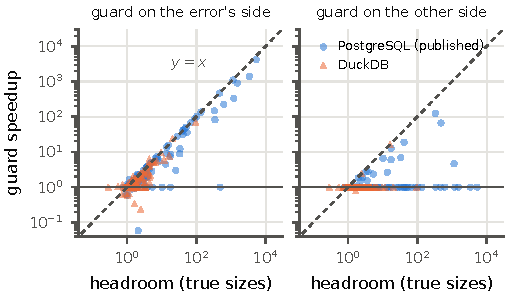
\includegraphics[width=\columnwidth]{../../figures/icde_execution.pdf}
\Description{Two log-log scatter plots with one point per STATS-CEB query for the published PostgreSQL estimates and for DuckDB: the speedup of a guard against the headroom of planning on the true sizes, with the diagonal for full recovery and a horizontal line at no change; left, the guard on the side the source mostly errs on; right, the other guard.}
\caption{Per STATS-CEB query (146), the speedup of a guard over the source's
injected estimates against the speedup of planning on the true join sizes.
Left: the guard on the side the source mostly errs on (upper for the published
PostgreSQL estimates, floor for DuckDB); right: the other guard. Dashed: the
guard recovers all of the headroom; solid: it changes nothing. Plans that
time out are kept at 300\,s (capped runtimes; Section~\ref{sec:execution}); both
axes divide by the same baseline time, which by itself correlates them.}
\label{fig:execution}
\end{figure}

\begin{table}[t]
\centering
\caption{Executed STATS-CEB plans in PostgreSQL: geometric-mean speedup over
each source's own injected estimates (146 queries, one row each; 95\%
query-clustered intervals; $\tau{=}1$; times capped at 300\,s). Planning on $\hat L$ needs a sample of
every sub-plan, so it is compared with the headroom on the 128 queries where
every sampled count finished.}
\label{tab:execution}
\scriptsize
\setlength{\tabcolsep}{2pt}
\begin{tabular}{@{}lrrr@{}}
\toprule
Policy & PG (published) & DuckDB & PG (ours) \\ \midrule
True join sizes & 4.38 [3.28, 6.01] & 1.70 [1.52, 1.92] & 1.35 [1.23, 1.51] \\
Upper guard & 3.08 [2.35, 4.15] & 1.02 [1.00, 1.07] & 1.02 [1.00, 1.05] \\
Sound floor & 1.21 [1.09, 1.36] & 1.39 [1.25, 1.56] & 1.05 [1.00, 1.13] \\
Both guards & 3.44 [2.62, 4.60] & 1.41 [1.28, 1.59] & 1.07 [1.02, 1.15] \\
Upper $+$ $\hat L$ floor & 3.59 [2.75, 4.80] & 1.69 [1.51, 1.90] & 1.18 [1.11, 1.28] \\
Plan on LpBound & 3.54 [2.70, 4.75] & 1.37 [1.21, 1.57] & 1.09 [1.00, 1.20] \\
\multicolumn{4}{@{}l}{\emph{128 queries with a complete sample}} \\
True join sizes & 3.59 [2.71, 4.89] & 1.70 [1.51, 1.94] & 1.30 [1.18, 1.49] \\
Plan on $\hat L$ & 3.57 [2.70, 4.87] & 1.69 [1.50, 1.94] & 1.30 [1.17, 1.48] \\
\bottomrule
\end{tabular}
\end{table}

\subsection{Planning on the sample}
On STATS-CEB a sampled count times out (120\,s) on at least one sub-plan of 18
queries, so we compare planning on $\hat L$ with the headroom on the other 128
(Table~\ref{tab:execution}, lower block). There it recovers all of the
headroom from every source: $3.57\times$ of $3.59\times$, $1.69\times$ of
$1.70\times$ and $1.30\times$ of $1.30\times$, and against the true sizes it is
indistinguishable ($0.99\times$). The 18 excluded queries are where the
headroom is: $17.83\times$ [5.79, 58.89] for the published PostgreSQL
estimates, against $3.59\times$ on the rest. A sample that does not finish
recovers nothing there; dividing the $\hat L$ speedup by the headroom over all
146 queries, as we first did, would understate what the sample achieves where
it exists and hide where it does not. Planning on LpBound, pessimistic
optimization's input, does worse: it runs $0.81\times$ [0.76, 0.86] as fast as
planning on the true sizes (44\% of queries slower) and only $1.09\times$ as
fast as our own optimizer's estimates; the artifact's own runs do not show
this slowdown on STATS-CEB (Section~\ref{sec:replication}).

These are planning results; the sample's cost is not charged. It is not small.
Timed in the same run, back to back with the query, sampling every sub-plan of
a query takes a median $2.68\times$ [1.87, 3.84] the time of executing the query
with our optimizer's plan, and longer than the query on 73\% of 127 queries.
These 127 exclude 19 queries whose native plan (3) or one of whose samples (16)
timed out, which are the most expensive to sample; keeping the timed-out
samples at their 120\,s cap raises the median to $3.31\times$ (76\% of 143
queries). Sampling every sub-plan for every query is therefore not affordable;
Section~\ref{sec:certificates} simulates sampling only the sub-plans that decide
the plan.

\subsection{JOB-light: five sources}
On JOB-light (Table~\ref{tab:execution-jl}) injection reproduces our
optimizer's native plan on every query and every sampled count finishes. Five
sources span both directions of error. The published PostgreSQL estimates now
\emph{underestimate} (97\% of queries, Section~\ref{sec:cardinality}) and the
roles of the guards swap: the floor recovers $1.38\times$ [1.16, 1.66] of a
$1.94\times$ headroom, the upper guard only $1.06\times$; against the native
plans, the floored plans reach $0.79\times$ [0.69, 0.91]. FactorJoin, which
overestimates (1\% of queries under), is the mirror image: the upper guard
recovers $1.18\times$ of $1.34\times$ and the floor changes no plan. BayesCard
leaves no headroom ($1.00\times$), and no sound guard changes any of its plans.
DuckDB is the exception to a clean reading: it underestimates on 83\% of
JOB-light queries, yet gains about as much from the upper guard
($1.10\times$ [1.02, 1.20]) as from the floor ($1.08\times$ [1.01, 1.16]);
with a headroom of $1.33\times$, its errors are moderate on both sides.
Planning on $\hat L$ again matches the true sizes for every source
($1.00\times$ against them), and planning on LpBound is again slower than
planning on the true sizes ($0.87\times$ [0.81, 0.92]). FactorJoin and
BayesCard are absent from STATS-CEB because their published sub-plan files
there cover only 1{,}499 of the 2{,}577 sub-plans, with conflicting duplicate
values for 671 and 776 entries; only 5 of 146 queries could be injected
completely.

\begin{table*}[t]
\centering
\caption{Executed JOB-light plans in PostgreSQL, as in
Table~\ref{tab:execution} (70 queries; every sampled count finished; times
capped at 300\,s).}
\label{tab:execution-jl}
\footnotesize
\setlength{\tabcolsep}{4pt}
\begin{tabular}{@{}lrrrrr@{}}
\toprule
Policy & PostgreSQL (published) & DuckDB & FactorJoin & BayesCard & PostgreSQL (ours) \\ \midrule
True join sizes & 1.94 [1.55, 2.48] & 1.33 [1.19, 1.52] & 1.34 [1.20, 1.53] & 1.00 [0.99, 1.03] & 1.12 [1.04, 1.24] \\
Upper guard & 1.06 [0.99, 1.15] & 1.10 [1.02, 1.20] & 1.18 [1.10, 1.28] & 1.00 [1.00, 1.00] & 1.01 [1.00, 1.02] \\
Sound floor & 1.38 [1.16, 1.66] & 1.08 [1.01, 1.16] & 1.00 [1.00, 1.00] & 1.00 [1.00, 1.00] & 1.08 [1.00, 1.19] \\
Both guards & 1.44 [1.22, 1.73] & 1.18 [1.07, 1.32] & 1.18 [1.10, 1.28] & 1.00 [1.00, 1.00] & 1.09 [1.01, 1.20] \\
Upper $+$ $\hat L$ floor & 1.87 [1.49, 2.40] & 1.31 [1.17, 1.50] & 1.18 [1.10, 1.28] & 1.00 [0.99, 1.02] & 1.12 [1.03, 1.24] \\
Plan on LpBound & 1.69 [1.38, 2.11] & 1.15 [1.01, 1.34] & 1.16 [1.07, 1.27] & 0.87 [0.81, 0.93] & 0.97 [0.90, 1.06] \\
Plan on $\hat L$ & 1.95 [1.56, 2.49] & 1.33 [1.19, 1.52] & 1.35 [1.20, 1.53] & 1.01 [0.99, 1.03] & 1.13 [1.04, 1.25] \\
\bottomrule
\end{tabular}
\end{table*}
\subsection{Against the artifact's own runs}
\label{sec:replication}
The LpBound artifact also reports end-to-end runtimes: PostgreSQL planning on
each estimator's sub-plan values on its authors' instance.
Table~\ref{tab:replication} sets them beside ours, matching their PostgreSQL
runs with our instance's native, non-injected plans (since injecting its own
estimates does not move them, the headroom is the same as in
Table~\ref{tab:execution}). The headroom to the
true sizes reproduces on both benchmarks, with overlapping intervals
($1.28\times$ against $1.35\times$ on STATS-CEB, $1.21\times$ against
$1.12\times$ on JOB-light), and so do both LpBound comparisons on JOB-light.
On STATS-CEB neither does: the artifact finds planning on LpBound as fast as
planning on the true sizes ($1.02\times$ [0.95, 1.09]), where we find
$0.81\times$, and $1.30\times$ faster than PostgreSQL, where we find
$1.09\times$. The artifact's timings are also not capped at 300\,s. We have not isolated the cause; the
two instances differ in version (13.14 with upstream \texttt{pg\_hint\_plan}
there, 13.1 with the benchmark patch here), hardware, configuration and timing
protocol (means of five cold-started runs there, medians of three interleaved
runs here), so our finding that
planning on LpBound lags the true sizes holds for our configuration and for
JOB-light, not in general.

The comparison also explains the published PostgreSQL estimates: they are not
our instance's. On STATS-CEB they are a median $4.7\times$ our instance's own
in-context estimates of the same sub-plans ($20\times$ on two-relation
sub-plans), on JOB-light $0.33\times$, and their median sub-plan $q$-error is
15.0 against 1.90 for ours (8.4 against 1.76 on JOB-light). Injected into our instance,
whose base-table estimates stay its own, they act as a strongly biased
estimator, overestimating on one benchmark and underestimating on the other.
That makes them a clean test of the guards' direction, and it makes their
large headroom a statement about this estimator, not about PostgreSQL.

\begin{table*}[t]
\centering
\caption{End-to-end speedups (geometric mean, 95\% query-clustered
intervals) in the LpBound artifact's own runs and in ours. ``PostgreSQL'' is
each instance planning on its own estimates; for ours, its native,
non-injected plan. Our timings are capped at 300\,s, the artifact's are not.}
\label{tab:replication}
\footnotesize
\setlength{\tabcolsep}{6pt}
\begin{tabular}{@{}lrrrr@{}}
\toprule
 & \multicolumn{2}{c}{STATS-CEB} & \multicolumn{2}{c}{JOB-light} \\
\cmidrule(lr){2-3}\cmidrule(l){4-5}
Speedup & Artifact & Ours & Artifact & Ours \\ \midrule
PostgreSQL $\to$ true sizes & 1.28 [1.14, 1.46] & 1.35 [1.23, 1.51] & 1.21 [1.06, 1.41] & 1.12 [1.04, 1.24] \\
PostgreSQL $\to$ LpBound & 1.30 [1.16, 1.48] & 1.09 [1.00, 1.20] & 1.02 [0.88, 1.18] & 0.97 [0.90, 1.06] \\
True sizes $\to$ LpBound & 1.02 [0.95, 1.09] & 0.81 [0.76, 0.86] & 0.85 [0.74, 0.96] & 0.87 [0.81, 0.92] \\
\bottomrule
\end{tabular}
\end{table*}

\subsection{On PostgreSQL 16 (post-hoc)}
\label{sec:pg16}
To see whether the execution results belong to one old version, we repeated
the STATS-CEB run on PostgreSQL 16.15: a stock server with upstream
\texttt{pg\_hint\_plan} 1.6.2, the same data, planner settings and protocol, statistics
from its own \texttt{ANALYZE}, and JIT compilation off, as PostgreSQL 13.1 has
none. The benchmark patch we use to read in-context estimates exists for 13.1
only. On 16 we read them with a small extension that wraps the planner's join
search and reports the size of every join relation it builds; on 13.1 it
reproduces the patch's values on all 2{,}577 STATS-CEB and 696 JOB-light
sub-plans. Forcing a join order whose prefix is the sub-plan does not: the
planner sizes a join relation from the first split its search builds, a forced
order builds it from another split, whose choice of join clauses and rounded
input sizes give another estimate, and 1{,}052 of the 2{,}577 values differ by
more than one row. Injecting PostgreSQL 16's own estimates reproduces its native
plan on all 146 queries. Table~\ref{tab:pg16} sets the two versions side by
side. Our first PostgreSQL 16 run had JIT on; an independent review caught it,
and we repeated the run with JIT off, which barely moves the numbers (last
column). We had frozen six predictions for the first run midway through it (67
of 146 queries measured, per-query times visible in the log, no aggregate
computed; supplement), and four held. On STATS-CEB the pattern holds: guards
rescue the published estimates, planning on LpBound is slower than planning on
the true sizes on both versions (so the gap to the artifact's runs in
Section~\ref{sec:replication} is not a property of 13.1), and a tighter
synthetic bracket recovers more of the headroom than the real one. On
PostgreSQL 16 the sound guards on its own estimates gained
$1.14\times$ [1.04, 1.27] of a $1.40\times$ headroom (38\%, against 23\% on
13.1), above the $1.12\times$ we predicted; with one run per version we cannot
separate this difference from run-to-run variation. An $8\times$ synthetic bracket
recovers 47\% [27, 62] of the headroom (51\% with JIT on, where we predicted
less than half; on the JIT-off run that prediction holds, which we do not
count). In each run one plan reached the 8\,GB cap on temporary files we set
and counts as cut off; temporary files went to a SATA disk here and to NVMe on
13.1, and both containers were pinned to the same four cores, the 13.1 one idle
during these runs. Intervals for the 13.1 column are in
Table~\ref{tab:execution}, the last row of Table~\ref{tab:replication}, and, for the
synthetic shares, Section~\ref{sec:execution}.

\begin{table}[t]
\centering
\caption{STATS-CEB execution on PostgreSQL 13.1 and 16 (146 queries each).
Rows 1--4 and 7--8: geometric-mean speedup over the source's own injected
estimates; rows 5--6: share of our estimates' headroom recovered; last row:
planning on LpBound relative to the true sizes. PostgreSQL 16 with JIT off (the
primary run, 95\% query-clustered intervals) and on (the first run). One run
per column, times capped at 300\,s. Post-hoc.}
\label{tab:pg16}
\footnotesize
\setlength{\tabcolsep}{3pt}
\begin{tabular}{@{}lrrr@{}}
\toprule
 & 13.1 & 16 & 16, JIT on \\ \midrule
Our estimates $\to$ true sizes & 1.35 & 1.40 [1.23, 1.62] & 1.42 \\
Upper guard on our estimates & 1.02 & 1.07 [1.01, 1.17] & 1.07 \\
Floor on our estimates & 1.05 & 1.06 [1.01, 1.14] & 1.06 \\
Both guards on our estimates & 1.07 & 1.14 [1.04, 1.27] & 1.13 \\
Both, synthetic $k=2$ (share) & 71\% & 81\% [69, 89] & 81\% \\
Both, synthetic $k=8$ (share) & 36\% & 47\% [27, 62] & 51\% \\
Published PG: upper guard & 3.08 & 2.48 [1.96, 3.19] & 2.42 \\
DuckDB: floor & 1.39 & 1.44 [1.29, 1.62] & 1.45 \\
True sizes $\to$ LpBound & 0.81 & 0.82 [0.76, 0.89] & 0.81 \\
\bottomrule
\end{tabular}
\end{table}

\section{A Pre-registered Held-out Test}
\label{sec:heldout}
To test the post-hoc findings on data we had not seen, we pre-registered seven predictions before measuring a seeded random sample of 200 of the artifact's 1{,}000 JOB-range queries (range filters over the JOB-light tables; the registration, two addenda filed before the measurements and the code hashes are in the supplement). The registered exclusions removed 9 for a sub-plan without an exact count; 12 for fewer than three relations, leaving 179 queries for the certificates and 191 for the tightness sweep. After execution, with the final result in $C_{out}$, PostgreSQL's plan is certified within $2\times$ on 86.6\% of queries with no sample (C1, predicted at least 70\%: confirmed) and on 88.8\% with the sampled floor (C2, at least 80\%: confirmed); without the final result on 7.3\% without a sample (C3, at most 5\%: inconclusive) and on 35.8\% with it (C4, between 10\% and 70\%: confirmed); the certificate's soundness check held on every query (C5: confirmed). Under both synthetic guards on PostgreSQL's own estimates, the share of plans that change falls from 19.4\% at $k=2$ to 5.8\% at $k=16$ (C6, at least halving and never rising by more than 5 points: confirmed); planning on the true sizes lowered $C_{out}$ by only $1.03\times$, below the registered $1.05\times$, so C7 was not testable. Of the 6 testable predictions, 5 were confirmed. (Added after the results:) C5 checks our code rather than the data; of the five empirical predictions that were testable, four were confirmed and C3 was inconclusive: on JOB-range 7.3\% of plans are certified without the final result even without a sample, so the final result is the main but not the only source of these certificates. With 95\% query-clustered intervals, C1--C4 are 86.6\% [81.6, 91.6],
88.8\% [83.8, 93.3], 7.3\% [3.9, 11.2] and 35.8\% [29.1, 43.0]. The test is
narrow: JOB-range uses the same IMDb tables as JOB-light, the 179 certificate
queries have 3--5 relations (the sweep also includes 12 with two), the queries excluded for a timed-out count are the
expensive ones, which favours C1 and C2 (the rules apply to point estimates;
were all 9 uncertified, C1 and C2 would still be confirmed at 82.4\% and
84.6\%, while C3 would lie between 6.9\% and 11.7\% depending on those 9,
inconclusive or falsified), and C1, C2 and C6 follow closely from
the mechanism seen on the development data. It tests the certificate after
execution and the plan-change trend, not the tightness gain of
Section~\ref{sec:execution}, which C7 could not test.

\section{Lessons and Limitations}
\label{sec:lessons}

\subsection{Recommendations}
\looseness=-1
\emph{For evaluating a bound,} report it with the estimators it is meant to
guard and the direction of their errors. A pooled tail hides that an upper
bound cannot touch an estimator that underestimates on 97\% of queries
(Table~\ref{tab:direction}), and pooling also hides what tightness buys: the
tighter bound reaches estimators the looser one never touches. \emph{For
producing bounds,} aim at the width that changes plans: on PostgreSQL's own
STATS-CEB estimates, a bracket within $2\times$ of the truth recovered 71\% of
the headroom and one within $8\times$ 36\%, against 23\% for today's (a
synthetic, post-hoc experiment, Section~\ref{sec:execution}).
\emph{For deploying a guard,} measure the headroom to the true sizes first; no
guard's geometric mean exceeded it here (a reference, not a bound), and for PostgreSQL's own
estimates in our configuration it was $1.35\times$ on STATS-CEB and
$1.12\times$ on JOB-light, of which the sound guards recovered little. Where the estimator's
errors fall on both sides, pair the upper bound with a floor.
\emph{For using a sample,} plan on $\hat L$ rather than flooring with $L$ where
the sample finishes, budget for the sub-plans where it does not (they carried
the largest headroom), and confine sampling to the sub-plans that decide the
plan, as our offline simulation suggests (Section~\ref{sec:certificates}):
sampling them all usually costs more than running the query.
\emph{For certifying plans,} report the share of queries where the choice
matters, and pair the bracket with a lower bound: without one, no upper bound
certified anything before execution, and after it the plan's own exact sizes
serve as one.

\subsection{Lessons from our own pipeline}
\looseness=-1
Several of our earlier results did not survive; we report what caught them,
since the same checks apply to any study that injects or bounds cardinalities.
\emph{Cross-validate the ground truth.} Our first exact counter treated SQL
\textsc{null} as a value in join keys and in filters, inflating some STATS-CEB
counts by up to $97\times$; only agreement with an independent
truth exposed it, and every count is now checked against the artifact and, in
this paper, against PostgreSQL (2{,}510 of 2{,}510). The same defect in our
degree statistics kept the max-degree bound sound but loosened it up to
$412\times$.
\emph{Check that a pre-registered criterion is attainable.} One rule of our
plan-certificate registration was unattainable because of the cost model's
symmetry, the other at our sample rate because of the floor's $1/r$ gap
(Section~\ref{sec:certificates}); checking both would have shown it before the run.
\emph{Measure cost in an engine.} The sampled lower bound costs $0.33\times$ the
exact count inside PostgreSQL and $0.66\times$ in our single-threaded Python
counter; the latter led us to call it ``never cheap''.
\emph{Divide by the same queries.} Planning on $\hat L$ is defined only where
every sampled count finishes; an earlier execution table of ours set its
speedup against the headroom over all queries, including 18 on which the
headroom for the published PostgreSQL estimates is more than four times that on
the rest, and so mixed two populations
(Section~\ref{sec:execution}).
\emph{Time what you compare in one run.} The same table combined runs taken
days apart on a shared host; every execution table here comes from a single
run per benchmark that covers all sources and policies.
\emph{Check that a hint is obeyed.} Our first execution of certified plans
used \texttt{pg\_hint\_plan}'s \texttt{Leading} hint, which our patched
PostgreSQL reported as used but did not follow; the plans it ran were not the
certified ones, and the certified orders appeared to run at a quarter of
PostgreSQL's speed. Forced with explicit joins and checked against the order,
they run as fast as PostgreSQL's own plans.
\emph{Read estimates in context.} We first read PostgreSQL's sub-plan estimates
from a separate \texttt{EXPLAIN} of each sub-plan; inside the full query the
planner sizes the same joins differently, and injecting the stand-alone values
reproduced its plan on only 90 of 146 queries, against 143 with the in-context
values.

\subsection{Limitations}
\label{sec:limitations}
\looseness=-1
The execution results come from one engine, PostgreSQL, in two versions (13.1
throughout; 16 for the STATS-CEB execution of Section~\ref{sec:pg16}, with its
own statistics and an 8\,GB cap on temporary files), two benchmarks and a shared
host, in one run per benchmark and version (and a JIT-on run on PostgreSQL 16).
To measure run-to-run variation we re-ran 61 STATS-CEB queries on 13.1 (21 certified
where the choice matters, 40 drawn by stratum) in six blocks hours
apart, restarting the server and randomizing the plan order in every round,
with predictions registered beforehand: a block's native plans ran up to
$1.25\times$ slower than their mean over blocks, yet all six predictions held
and every ratio stayed within 6\% of the main run on the same queries (both guards $1.04\times$, true
sizes $1.31\times$, certified plans $1.37\times$, or $0.35\times$ with same-block
sampling; supplement). The load gate checks a query's start only (on PostgreSQL 13.1 the
highest start load was 59.8; two STATS-CEB queries ended above 60, at most
64.8), and plans cut off at
300\,s (on 13.1, 25 on STATS-CEB; 11 on JOB-light, all of one query on which
every plan times out; on 16, 24 with JIT off) make the speedups ones of capped
runtimes, of unknown direction where two different plans time out. Planning on $\hat L$ is compared on the 128 STATS-CEB
queries where the sample finishes, a subset we chose after seeing that the
other 18 carry most of the headroom. Of the lower-bound producers we evaluate
only the sample; statistics-based lower bounds such as
xBound~\cite{stoian2026xbound}, which cost no execution, are not covered, nor are
exact sizes counted by dynamic programming over a join tree without
enumerating the join~\cite{zhao2018sampling}.
Injecting PostgreSQL's own in-context estimates reproduces its plan on 143 of
146 STATS-CEB queries on 13.1 (146 on 16), and the ``true'' sizes cover join sub-plans only; on STATS-CEB our headroom
is smaller than that reported by Han et al.\ (Section~\ref{sec:execution}). The
estimators are those of the LpBound artifact at its configuration; we
retrained none, the published PostgreSQL estimates differ from our instance's,
and FactorJoin and BayesCard could be executed on JOB-light only. The
plan-certificate analysis uses $C_{out}$ and left-deep orders, defines
connected prefixes by explicit join predicates on STATS-CEB but by the
artifact's sub-plan list (which includes joins implied by key equalities) on
JOB-light, and was designed after its pre-registered predecessor failed. The analyses of
what makes a plan certifiable, of the oracle's sampling price and of certifying
after execution are post-hoc too, on data we had already analysed; we froze
predictions for them, and for one analysis reported only in the supplement,
before running them. Of the six predictions behind these post-hoc analyses, three
failed (the sound tightening, the oracle's price and the witness floor, the
last tested with a different $k$ than predicted; reported where they appear) and three held only in part; for the executed tightness
experiment the prediction concerned the upper guard alone, whose share of the
headroom never reached half, and the two-sided guard we report was chosen
afterwards. The guard funnel had no prediction. The held-out test
(Section~\ref{sec:heldout}) confirms only the certificate after execution and
the plan-change trend; the proposition's consequences, $\rho$, the oracle's
price, the witness floor and the 71\% have no confirmatory test. Its
registration and addenda were frozen and hashed before the measurements but,
like the earlier one, have not been deposited with a public registry. The sample's cost
is charged per sub-plan, not amortized across queries, which a deployment
might do, and the costs of selective sampling and of the certified plans with
their sampling combine sample times from the sampling run with execution times
from the execution runs, which time the same native plans $1.24$--$1.33\times$
apart on average, enough to move the cost of sampling every sub-join from below
the query's time to above it. The certificate computation, which compares every
pair of left-deep orders, took a median 1.2\,ms and at most 160\,ms per query
in the re-measurement, and every bracket assumes the data do
not change between sampling, bounding and execution; with updates, a deployment
would need a snapshot or a refresh.
\section{Conclusion}
\label{sec:conclusion}
On both benchmarks, what a sound bound bought depended on the estimator it
met. Guards repair the direction they see, and estimators err in
different directions; a tighter bound reaches more of them; and the
sample behind a lower bound is a better estimate than any guard makes. Plan
certificates become possible once a consumer accounts for what plans share and
a lower bound is present, a finding we reached only after our pre-registered
criterion failed; on STATS-CEB the plans they certify with the 10\% sample run
as fast as PostgreSQL's own, and faster where the choice matters; the sample, not plan
quality, is what certification costs, and among the samples we measured no
choice of which to take changed that. In a real optimizer, the same guard that rescues a strongly biased
estimator changes little for PostgreSQL's own, and the reason is width, not
visibility: the bracket sees most of its large errors, but in a synthetic
experiment only a bracket a few times wide moved enough plans. On held-out
JOB-range queries, a pre-registered test confirmed that PostgreSQL's executed
plans are mostly certifiable after the fact and that looser brackets change
fewer plans; whether the shared final result is nearly their only source (C3)
stayed inconclusive. On PostgreSQL 16 (STATS-CEB) the pattern held; guards
on its own estimates gained more than we predicted, in a single run. For the bound literature the
consequence is to evaluate a bound against the estimator and consumer it will
meet; for practitioners, to measure the headroom to the truth first, since in
our runs no guard recovered more on average, though it is no bound.

\section*{Acknowledgment of AI Use}
\looseness=-1
We used Anthropic's Claude models, through the Claude Code agent, throughout
this work, at the following levels. \emph{Code (Sections~\ref{sec:setup}--\ref{sec:heldout}):} the
measurement harness, the analysis and statistics scripts, the tests and the
figure scripts were written by the assistant at the author's direction and
reviewed by the author; the results are regenerated from the released code,
and an automated check confirms that each headline number and generated table
row appears in the text. \emph{Text (all sections):} drafts and revisions of every section
were produced with the assistant and edited and approved by the author.
\emph{Literature (Section~\ref{sec:related}):} an assistant agent retrieved bibliographic
records from dblp and Crossref, and we kept only entries whose retrieved record
matched. \emph{Internal review:} we used the assistant to simulate strict
reviewers and independent auditors of the code, data and text; several defects
reported in Section~\ref{sec:lessons} were found this way. These simulated reviews are not
peer review and are not reported as such. The assistant proposed analyses and
wording; the author chose the research questions, benchmarks and estimators,
decided which analyses to run and report, and is responsible for all content.

\section*{Artifacts}
\looseness=-1
Code, results and provenance are public at
\url{https://github.com/suanlab/sound-bounds-in-practice} (MIT licence; the
submitted version is tagged \texttt{pvldb2027-submission-r6} and includes
the paper's source). They comprise the harness (sub-plan counting and sampling
inside PostgreSQL, injection through \texttt{pg\_hint\_plan}, the certificate
computations), every per-query result as JSON, and the analysis scripts.
\texttt{docs/vldb\_2027/REPRODUCE.md} leads to a map from each number in the
paper to the command that produces it, and \texttt{audit\_icde\_numbers} re-derives the headline numbers
from the results and checks them against the \LaTeX{} source. Re-running needs
the public STATS and IMDb data, the LpBound artifact~\cite{zhang2025lpbound}
for estimates and truth, and the STATS-CEB benchmark's PostgreSQL
patch~\cite{han2021cardest}, built by a Dockerfile we include; PostgreSQL 16 is
a stock server with the \texttt{joinrel\_log} extension, also with its
Dockerfile. Third-party code and data are referenced, not redistributed, except
the held-out JOB-range sub-plan list, a subset of the LpBound artifact's (MIT
licence).

\bibliographystyle{ACM-Reference-Format}
\bibliography{../references}

\end{document}
